\chapter{Parameter Inference with Bifurcation Diagrams}
\label{chapter:inference}
\epigraph{``No person will deny that the highest degree of attainable accuracy is an object to be desired, and it is generally found that the last advances towards precision require a greater devotion of time, labour, and expense, than those which precede them."}{Charles Babbage}

\section{Preface}
\begin{enumerate}
    \item How does this paper address limitations of Chapter \ref{chapter:double-exclusive} 
    \item Alternative approaches
\end{enumerate}

In this section a single iteration of the model reduction loop
outlined in Section \ref{section:refinement}
is bench-marked against synthetic data that represent noisy single cell
gene expression trajectory data. The results show how one could start
with a hypothesis containing 30 parameters, and end up with only
7 relevant parameters after one iteration.

\subsection{Synthetic Data Generation}
The Euler-Maruyama method is used to generate $N/K$ points per
trajectory for $K$ trajectories  from a ground truth field $\Vector{g}$ with a
specific signal to noise ratio $\alpha$. The dataset 
$\mathcal{D}=\{\Vector{u}_1^1\dots\Vector{u}_{N/K}^K\}$ is obtained by
\vspace{-1em}
\begin{align}
    \Vector{u}_{n+1}^k =
    \Vector{u}_{n}^k +\Vector{g}(\Vector{u}_{n}^k)\Delta t
    +\frac{1}{\alpha}|\Vector{g}(\Vector{u}_{n}^k )|\Delta W\\
    \text{for given initial conditions}\quad\Vector{u}_{1}^1 \dots \Vector{u}_{1}^K\nonumber\\
    \Delta W \sim \mathcal{N}(0,\sqrt{\Delta t})\qquad\qquad
\end{align}
where $\Delta t$ is a sufficiently small chosen timestep, and $\Delta W$ is a Wiener
process, distributed normally with a mean of zero and standard deviation of $\Delta t$.
Figure \ref{fig:sample-data} shows example data generated from uniform cycle field
\begin{equation}
    \Vector{g}(x,y)=\frac{1}{\sqrt{x^2+y^2}}
    \begin{pmatrix}
    -y \\ x
    \end{pmatrix}
    \label{eq:cycle-field}
\end{equation}
\vspace{-2em}
\begin{Figure}
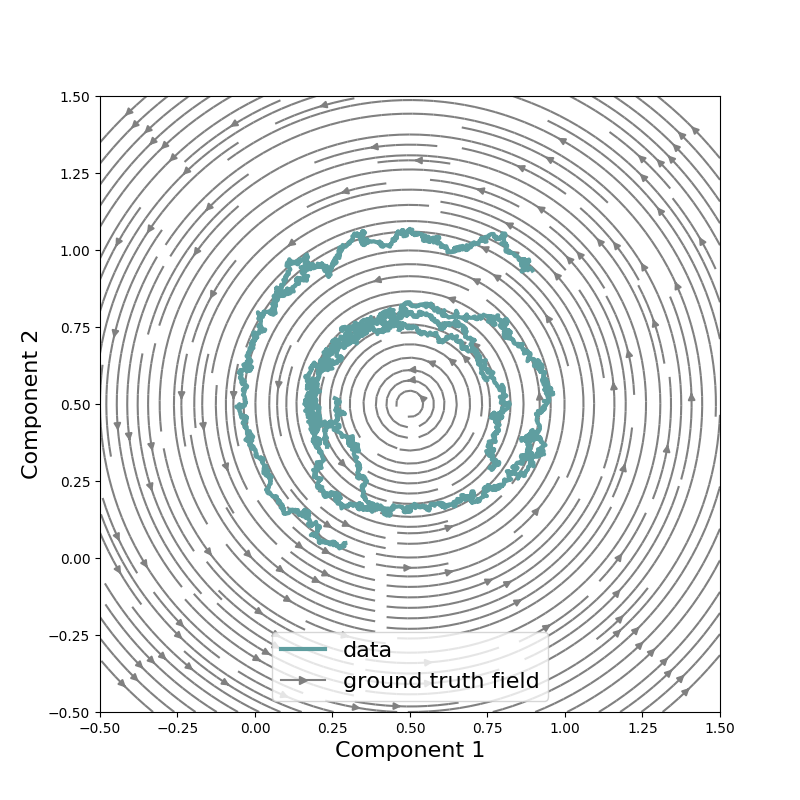
\includegraphics[width=70mm]{figures/sample-data-2.png}
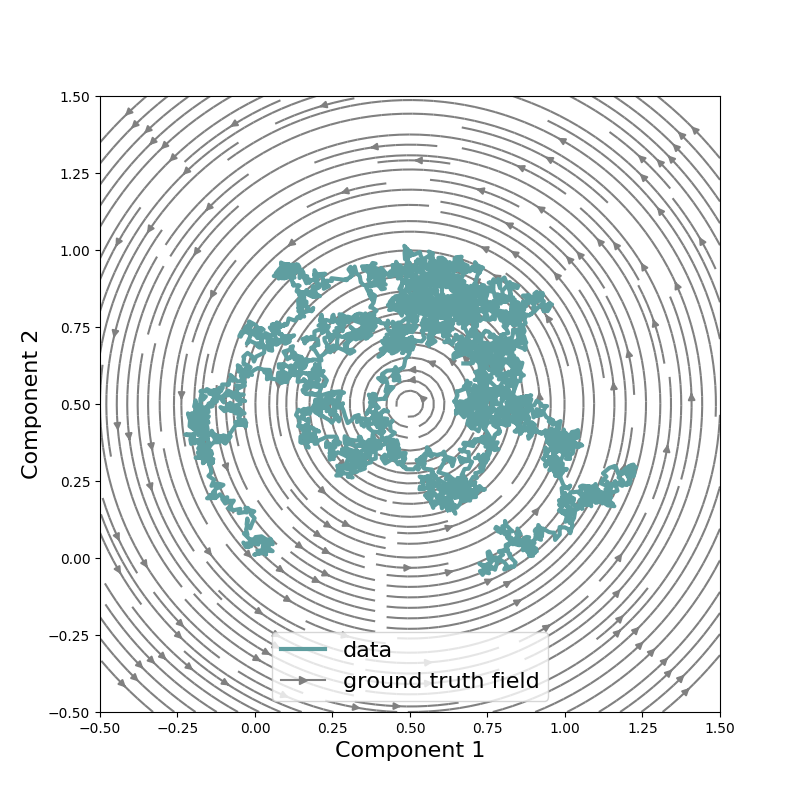
\includegraphics[width=70mm]{figures/sample-data-3.png}
\caption{\textcolor{Emerald}{Datasets} $\mathcal{D}$ generated from cycle field \eqref{eq:cycle-field}
for $K=7$ initial \\conditions. Signal to noise ratios are $\alpha=10,\sqrt{10}$
on left, right respectively}
\label{fig:sample-data}
\end{Figure}

\subsection{Non-parametric Inference with Gaussian Processes}
A non-parametric estimate of the vector field $\Vector{f}(\Vector{u})$ can be
obtained by assuming $\mathcal{D}$ is generated by a Gaussian process.
This requires the inversion of an $N\times N$ data matrix which has a computational
complexity $N^3$ which is only tractable with sparse datasets. Since top-down
feature specification is indeed sparse and it is always possible to partition
and down-sample larger datasets, this approach is appropriate for our given
objectives. Let the region $\partial\mathcal{D}$ be defined by the Delaunay tessellation of the
input data $\mathcal{D}$. The inferred field is defined only within the region
$\partial\mathcal{D}$ to minimise basis function artefacts.
\begin{equation}
    \Vector{f}(\Vector{u})\sim
        \mathcal{N}(\,\Vector{\mu}(\Vector{u}) ,\Matrix{\Sigma}(\Vector{u})\,)
    \quad\mathrm{for}\quad\Vector{u}\in\partial\mathcal{D}
\end{equation}\\
where at any given state $\Vector{u}$ the field is generated by Gaussian
distributions of mean vector $\Vector{\mu}(\Vector{u})$ and covariance matrix $\Matrix{\Sigma}(\Vector{u})$.
Solving for these requires a choice of matrix-valued kernel function $\Matrix{K}(\Vector{u},\Vector{v})$
which encodes our knowledge about the local structure of the field.
Sophisticated kernels for learning vector fields exist \cite{Fuselier2017ADecompositions} for decomposing
fields in conservative and solonoidal components, which aid in localising fixed points and
limit cycles. The simplest choice of kernel assumes the components are independent
and have a finite correlation length $\gamma$, such as Gaussian radial basis functions.
Here $\Matrix{I}$ is the identity matrix and the hyperparameter $\gamma$ has to be optimised.
\begin{equation}
    \Matrix{K}(\Vector{u},\Vector{v}) = \Matrix{I}\,\mathbb{e}^{-\gamma|\Vector{u}-\Vector{v}|^2}
\end{equation}
The geometric error $E$ between the inferred field $\Vector{f}$ and the ground truth $\Vector{g}$ at a specific
location in state space $\Vector{u}$ is a quatifty that should be zero
when the fields are pointing in the same direction and one when they are pointing in opposite
directions. Hence the use of the dot product
\begin{align}
    E(\Vector{f}|\Vector{g}) :=
    \frac{1}{2}
    \left(1-\frac{\Vector{f}\cdot\Vector{g}}{|\Vector{f}||\Vector{g}|}\right)\qquad\qquad\quad\\
    = \frac{1-\cos\theta}{2}\quad\text{where $\theta$ is the angle between $\Vector{f}$ and $\Vector{g}$}
\end{align}
Figure \ref{fig:inferred-cycles} shows inferred fields using the
$\pythoninline{GaussianProcessRegressor()}$ class from $\pythoninline{sklearn}$
\cite{Seeger2004GaussianLearning.} from data generated from \eqref{eq:cycle-field}.
Its clearly visible the field inference fails outside the data region $\partial\mathcal{D}$,
justifying the desire to only define the inferred result within the region. It can
also be seen that data generated with a lower signal-to-noise ratio $\alpha$ may
results larger geometric mismatches within the data region. Figure \ref{fig:inferred-at-snr}
reveals the robustness of this proceedure with respect to noise, showing a
consistent mean error below $16\%$. However this does not necessarily mean that
global dynamics are of the inferred field match that of the ground truth. In the
right sub-figure of Figure \ref{fig:inferred-cycles} it can be seen that the noisy
trajectories induce a stable fixed point at their centre.

\begin{Figure}
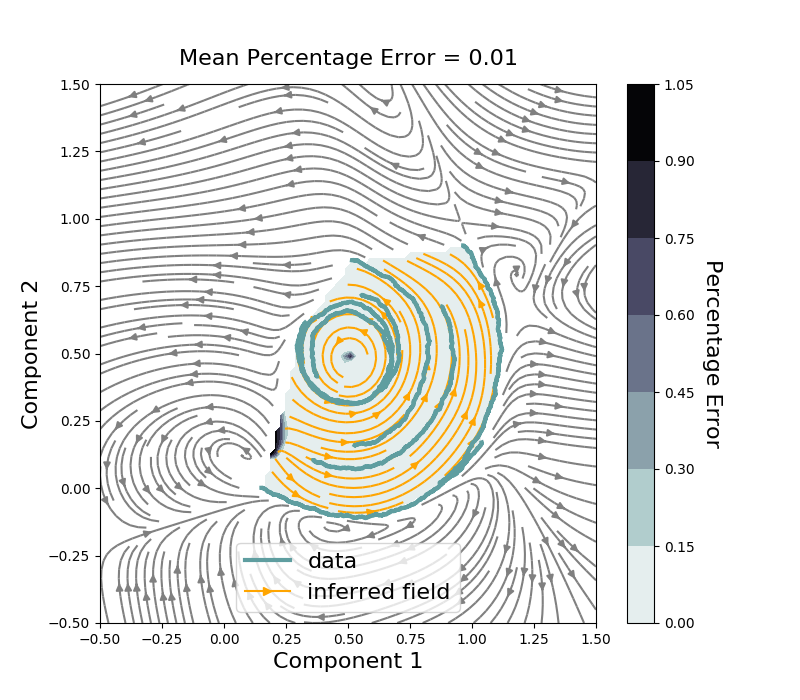
\includegraphics[width=70mm]{figures/cycle-2.png}
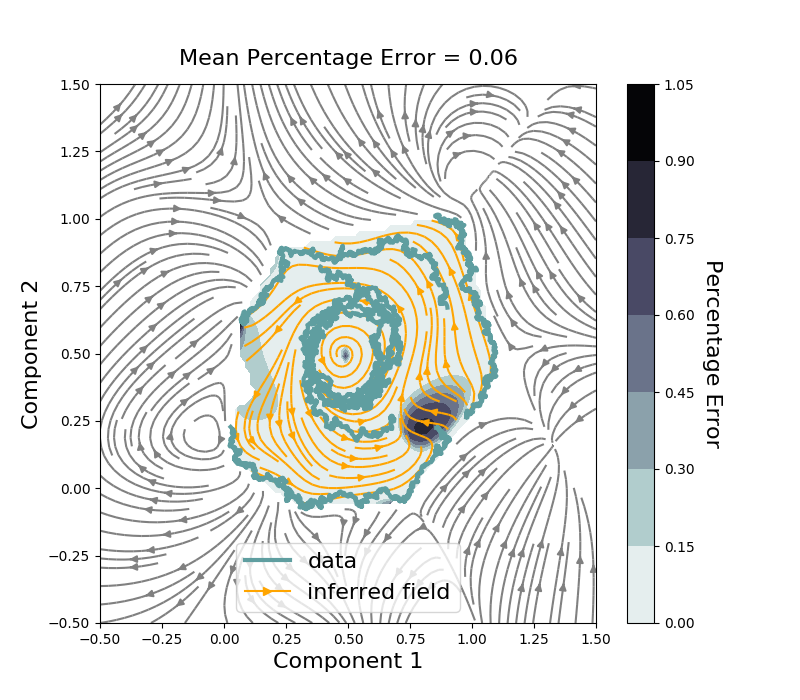
\includegraphics[width=70mm]{figures/cycle-1.png}
\caption{Gaussian process regressors inferring fields from \textcolor{Emerald}{cycle data} $\mathcal{D}$ with varying signal to noise ratios. Error $E$ is shown as a heatmap on \textcolor{orange}{inferred fields}  $\Vector{f}$ 
within the data region $\partial\mathcal{D}$.}
\label{fig:inferred-cycles}
\end{Figure}
\vspace{-2em}
\begin{Figure}
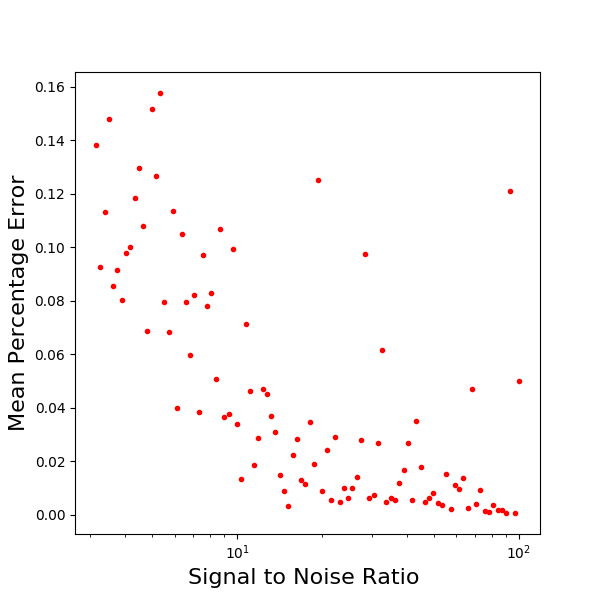
\includegraphics[width=80mm]{figures/cycle-snr.png}
\caption{Mean geometric error of the inferred field $\Vector{f}$ as a function\\
of signal-to-noise ratio $\alpha$ used to generate data $\mathcal{D}$}
\label{fig:inferred-at-snr}
\end{Figure}

\subsection{Geometric Inference of Parameters}
Suppose an accurate non-parametric representation $\Vector{f}$ of the observations
$\mathcal{D}$ or top-down specified hypothesis $\mathcal{H}$ has been obtained.
This section outlines a method by which parametric hypotheses
$\Vector{h}(\Vector{\theta})$ can be matched to $\Vector{f}$, and to what extent
parameters $\Vector{\theta}$ are relevant in matching the it. In order to
to this the following geometric cost function $\mathcal{L}(\Vector{\theta})$ must
be minimised
\begin{align}
    \mathcal{L}(\Vector{\theta}) &:= \mathbb{e}^{E(\Vector{f}|\Vector{h}(\Vector{\theta}))}
    +\lambda ||\Vector{\theta}||\\
    &= \sqrt{\mathbb{e}}\,
    \mathbb{e}^{-\frac{\Vector{f}\cdot\Vector{h}(\Vector{\theta})}
    {|\Vector{f}||\Vector{h}(\Vector{\theta})|}}
    +\lambda ||\Vector{\theta}||
\end{align}
where $\lambda$ is a regularisation hyperparameter and $||\Vector{\theta}||$ is some
norm with respect to the parameters. This norm encodes our prior assumptions on
what parameters we expect to find or wish to find. To reduce the complexity of
the inferred hypothesis, it should be assumed that as many parameters as possible
are zero. This can be done by choosing the $\ell_1$ norm for regularisation. Suppose
the hypothesis takes a mass-action form, then one could express the field as
\begin{equation}
    \Vector{h}(\Vector{\theta})=\Matrix{\Theta}\,\Vector{\phi}
    \quad\text{where}\quad\Vector{\phi}:=(u_1, u_2, u_1 u_2, u_1^2\,...\, )
\end{equation}
where the the parameter matrix $\Matrix{\Theta}$ multiplies a polynomial feature
vector $\Vector{\phi}$. Figure \ref{fig:convergence} shows a convergening optimisations
of $\mathcal{L}(\Vector{\theta})$ for the above hypothesis $\Vector{h}(\Vector{\theta})$
against the ground truth field given by \eqref{eq:cycle-field} using $\pythoninline{scipy.optimize.minimize(method='SLSQP')}$. It is possible to identify sloppy
vs stiff parameters by ordering them according to their variance from model to model.
Most parameters are stiff and zero as set by the regularisation, leaving non-zero
parameters which are either stiff or sloppy. Upon closer inspection of the sloppy
parameters $\Vector{s}\in\Vector{\theta}$ it can be deduced that 
\begin{equation}
    \Vector{z}=\Matrix{W}\,\Vector{s}
\end{equation}
where $\Matrix{W}$ is a sparse rectangular matrix that constructs linear combinations
of sloppy parameters to minimise the variance of the output $\Vector{z}$. There are
several decomposition algorithms that one could use to obtain this matrix $\Matrix{W}$
such as Independent Component Analysis. Figure \ref{fig:indepedent} reveals that
the terms indeed are only sloppy to preserve their sums or differences. Out of 30
parameters inferred this procedure suggests that only 7 of them are relevant for
model construction.

\begin{Figure}
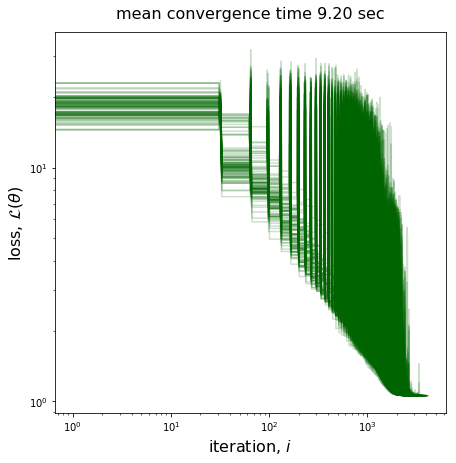
\includegraphics[width=70mm]{figures/convergence.png}
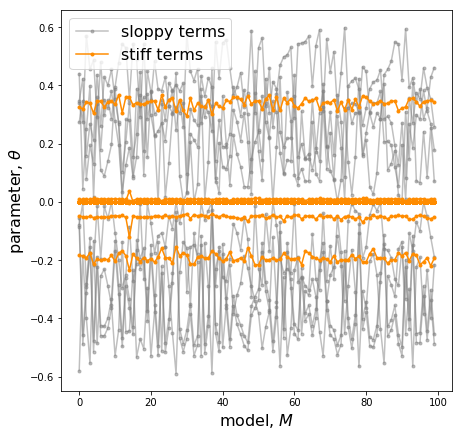
\includegraphics[width=70mm]{figures/parameters.png}
\caption{Left: convergence loss minimisation $\mathcal{L}(\Vector{\theta})$ for 100 initialisations of
of the parameter vector $\Vector{\theta}$ Right: Final parameters for each obtained model,
revealing sloppy and stiff terms}
\label{fig:convergence}
\end{Figure}

\begin{Figure}
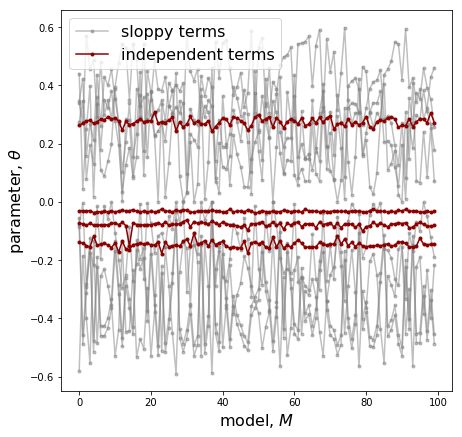
\includegraphics[width=70mm]{figures/indepedent.png}
\caption{Independent component analysis applied to the sloppy terms $\Vector{s}$.\\
The independent terms are either sums or differences of the sloppy terms.}
\label{fig:indepedent}
\end{Figure}
\newpage
\subsection{Basis Function Models}
Parametric models such as mass-action are can be expressed as
\begin{equation}
    \partial_t\Vector{u}(t) = \Matrix{\Theta}\,\Vector{\phi}(\Vector{u})
\end{equation}
the nullclines are
\begin{equation}
    \Matrix{\Theta}\,\Vector{\phi}(\Vector{u}) = 0
\end{equation}
suggesting isotropically re-scaling the parameters
doesn't change the location of the nullclines $\Matrix{\Theta}\rightarrow\alpha\Matrix{\Theta}$
where $\alpha$ is positive definite.

\subsection{Extending the Bifurcation Measure for Limit Cycles}

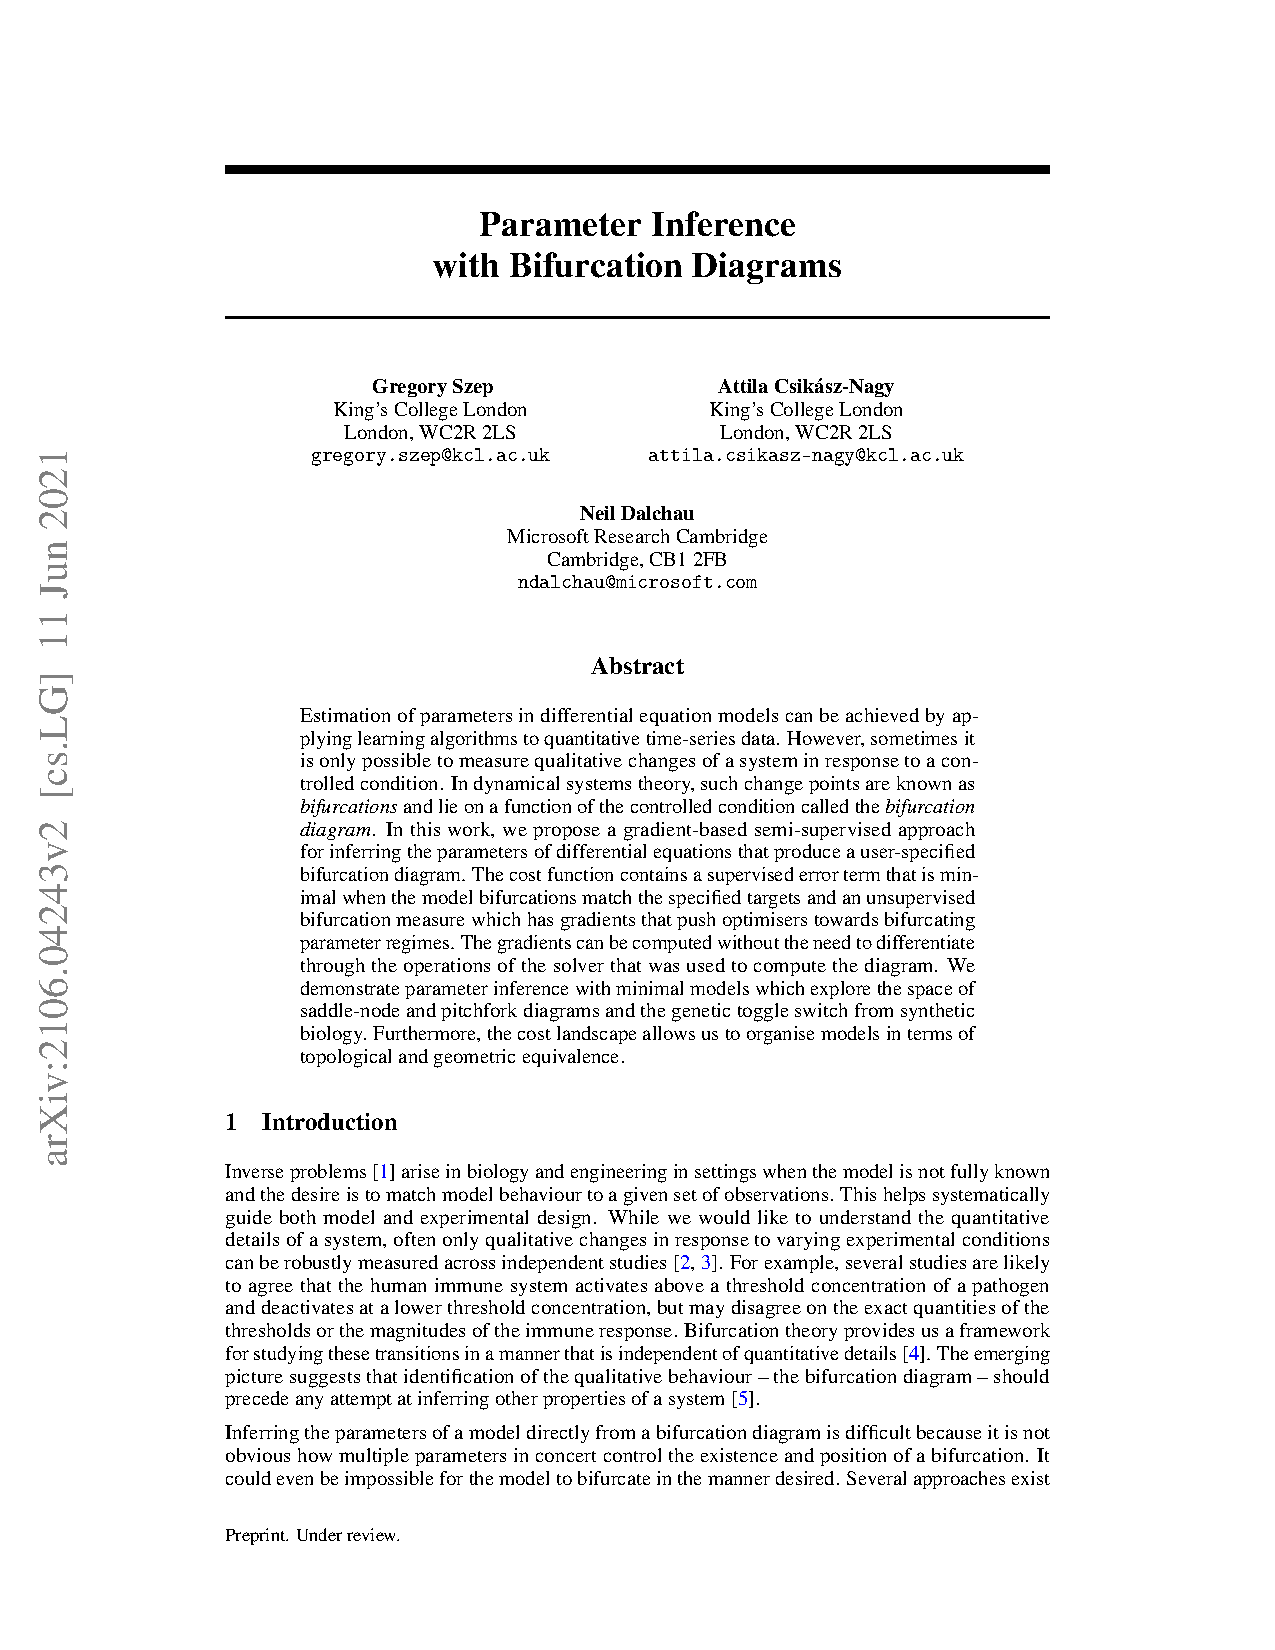
\includepdf[pages=1-11, offset=75 -95, scale=0.85, frame,
        clip,trim=31mm 21mm 31mm 21mm,
        pagecommand={}, addtotoc={
        1,section,1,Abstract,inference:abstract,
        1,section,1,Introduction,inference:introduction,
        2,subsection,2,Preliminaries,inference:preliminaries,
        4,section,1,Proposed Method,inference:method,
        4,subsection,2,Semi-supervised Cost Function,inference:cost,
        5,subsection,2,Differentiating the semi-supervised cost function,inference:derivatives,
        6,section,1,Experiments \& Results,inference:results,
        6,subsection,2,Minimal Models,inference:minimal,
        6,subsection,2,Genetic Toggle Switch,inference:genetic,
        7,subsection,2,Complexity,inference:complexity,
        9,section,1,Conclusion \& Broader Impact,inference:impact,
        9,section,1,Acknowledgements,inference:acknowledgements},
    addtolist={
        3, figure, {\textit{Fig. 1}\quad Illustration of bifurcation diagrams for minimal models of bifurcations. A. Saddle-node bifurcations arise for $\rates(u,p) = p + \theta_{1}u+\theta_{2}u^3$ when $\theta = (\frac{5}{2},-1)$. B. Pitchfork bifurcations arise for $\rates(u,p) = \theta_{1} + p u+\theta_{2}u^3$ when $\theta=(\frac{1}{2},-1)$. Targets are illustrated by light yellow vertical lines. Bifurcation curves are shown as solid blue and red lines, with lighter shades indicating the determinant crossing zero at locations $\predictions(\theta)$ giving rise to unstable solutions.}, figure:inference:minimal-models,
        4, figure, {\textit{Fig. 2}\quad Bifurcation measure $\measure(s)$ and determinant $\Det$ along the arclength $s$ of two different bifurcation curves demonstrating how maximising the measure along the curve maintains the existing bifurcation marked by a circle, while encouraging new bifurcations marked by stars.}, figure:inference:measure,
        7, figure, {\textit{Fig. 3}\quad Saddle-node $\rates(u,p) = p + \theta_{1}u+\theta_{2}u^3$ and pitchfork $\rates(u,p) = \theta_{1} + u p +\theta_{2}u^3$ optimised with respect to $\theta$ so that predicted bifurcations $\predictions(\theta)$ match targets $\targets$ in control condition $p$. The right panel shows bifurcations diagrams for the three optimal $\theta^*$ marked by stars on the left panel. The optimisation trajectories in white follow the gradient of the cost, approaching the black lines of global minima in the left panel}, figure:inference:minimal-models:results,
        8, figure, {\textit{Fig. 4}\quad Bifurcation inference for the two-state model (11). A. Optimal parameter estimates $\theta^*$ for the targets $\targets=\{4,5\}$ reveal two clusters of qualitatively different regimes: mutual activation ($a_1 < 1$; cluster 1) and mutual inhibition ($a_1 > 1$; cluster 2). B. Example bifurcation diagrams indicate positively and negatively correlated dependencies between the two model states, as a function of the control condition.}, figure:inference:two-state-optima,
        8, figure, {\textit{Fig. 5}\quad Complexity scaling of calculating the gradient of the cost function. Calculations were performed on an Intel Core i7-6700HQ CPU @ 2.60GHz x 8 without GPU acceleration}, figure:scaling
}]{publications/bifurcation-inference.pdf}